\section{이론적 배경}

\subsection{라즈베리파이}

라즈베리파이는 영국의 라즈베리파이 재단에서 개발한 초소형 컴퓨터 기판으로 학교 등에서 저가로 컴퓨터 교육을 할 수 있게 하기 위해 개발되었다. 하드 디스크 드라이브(HDD)와 솔리드 스테이트 드라이브(SSD)가 내장되어 있지 않으며 운영체제를 포함한 모든 파일은 마이크로 SD 카드에 저장된다. 본 연구에서 사용된 라즈베리파이의 모델은 Raspberry Pi 3 B이다. 라즈베리 파이 3에는 전원 공급 핀 4개, GND 핀 8개, UART 통신 핀 2개, GPIO 핀 24개 등 총 40개의 핀이 존재하며 이 핀을 통해 각종 센서들을 연결하여 센서에서 측정한 값을 프로그램을 통해 읽어들여 라즈베리파이의 디스플레이에 표시하거나 저장할 수 있다. 아날로그 핀이 존재하는 아두이노와는 달리 라즈베리파이의 GPIO 통신 핀은 모두 디지털 통신 방식을 사용한다는 차이점이 있다. 그 외에 4개의 USB 포트, HDMI 포트 등이 존재하며 전원은 5V의 직류 전압을 사용한다.

\begin{figure}[htbp]
	\centering
	
\includegraphics[width=.2\textwidth]{raspilogo}
	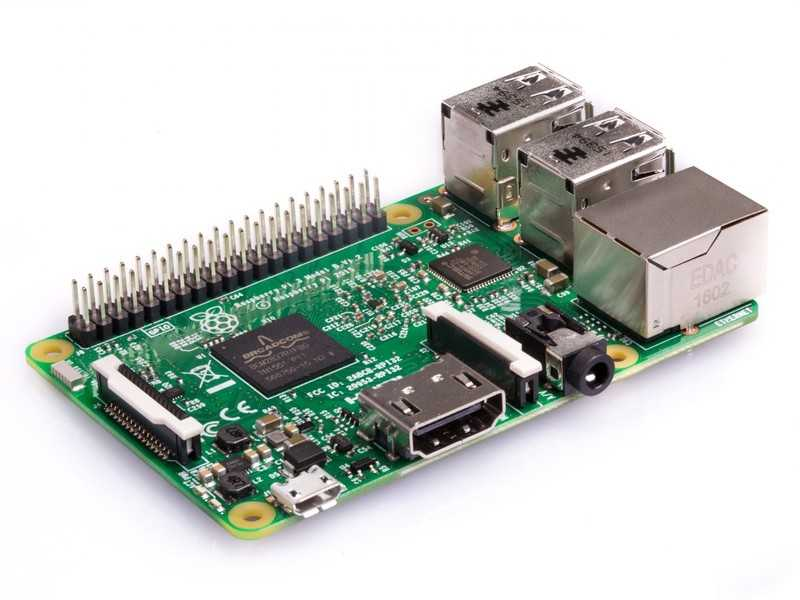
\includegraphics[width=.4\textwidth]{raspberrypi3b}
	\caption{Raspberry pi Logo와 본 연구에서 사용하는 3 B 모델}
	\label{RASPI}
\end{figure}

\subsection{라즈비안 (Raspbian)}
라즈비안은 라즈베리파이의 운영 체제(OS) 중 하나이며 라즈베리 파이 재단에서 개발한 공식 운영체제이다. 데비안 리눅스 기반의 운영 체제이며 프로그래밍을 편리하게 하기 위해 Python, Scratch 등의 프로그램을 미리 설치하여 배포하는 Raspbian with Desktop and Recommended Software 버전이 존재하며 연구에서 사용하였다. 2019년 11월 현재 라즈비안의 최신 버전은 4.19이며 본 연구에서는 최신 버전을 사용하였다.

\subsection{MariaDB}
MariaDB는 오픈소스 관계형 데이터베이스 관리 시스템(RDBMS, Relational Database Management System)이다. 사용하는 소스 코드의 기반이 MySQL과 같기 때문에 Python의 pymysql 모듈과 MySQL에서 데이터를 관리하기 위해 사용하는 코드인 SQL문을 사용해서 MariaDB 서버에 데이터를 전송할 수 있다.

\begin{figure}[htbp]
	\centering
	
\includegraphics[width=.4\textwidth]{mariadblogo.png}
	\caption{MariaDB 로고}
	\label{MariaDB}
\end{figure}

\subsection{AWS}
AWS는 컴퓨터를 통해 자동으로 기상 정보를 수집하는 장비이다. 기존의 유인 기상관측소에 비해 비용이 적게 들고 정확성이 높다는 장점이 있다. 대한민국 기상청에서는 전국에 500여 개의 AWS를 설치해 온도, 습도, 강수량, 강수 여부, 풍속, 풍향 등의 기상 요소를 수집하고 있으며 수집한 자료는 기상청 날씨누리에 모두 공개되고 있다.

\begin{figure}[htbp]
	\centering
	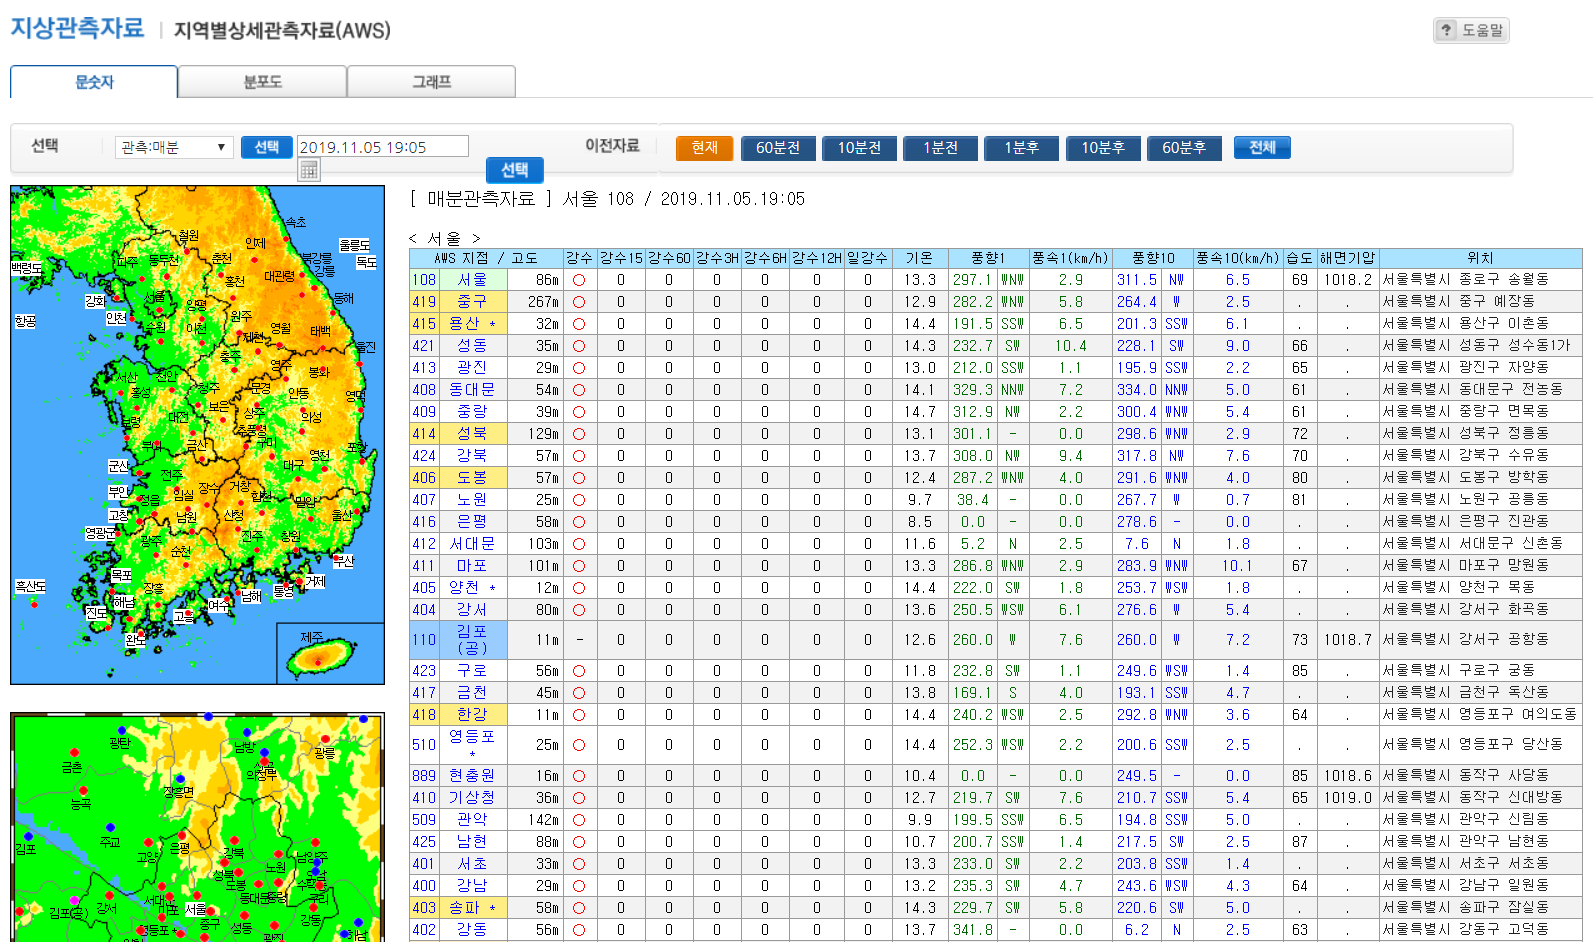
\includegraphics[width=.6\textwidth]{awsdata}
	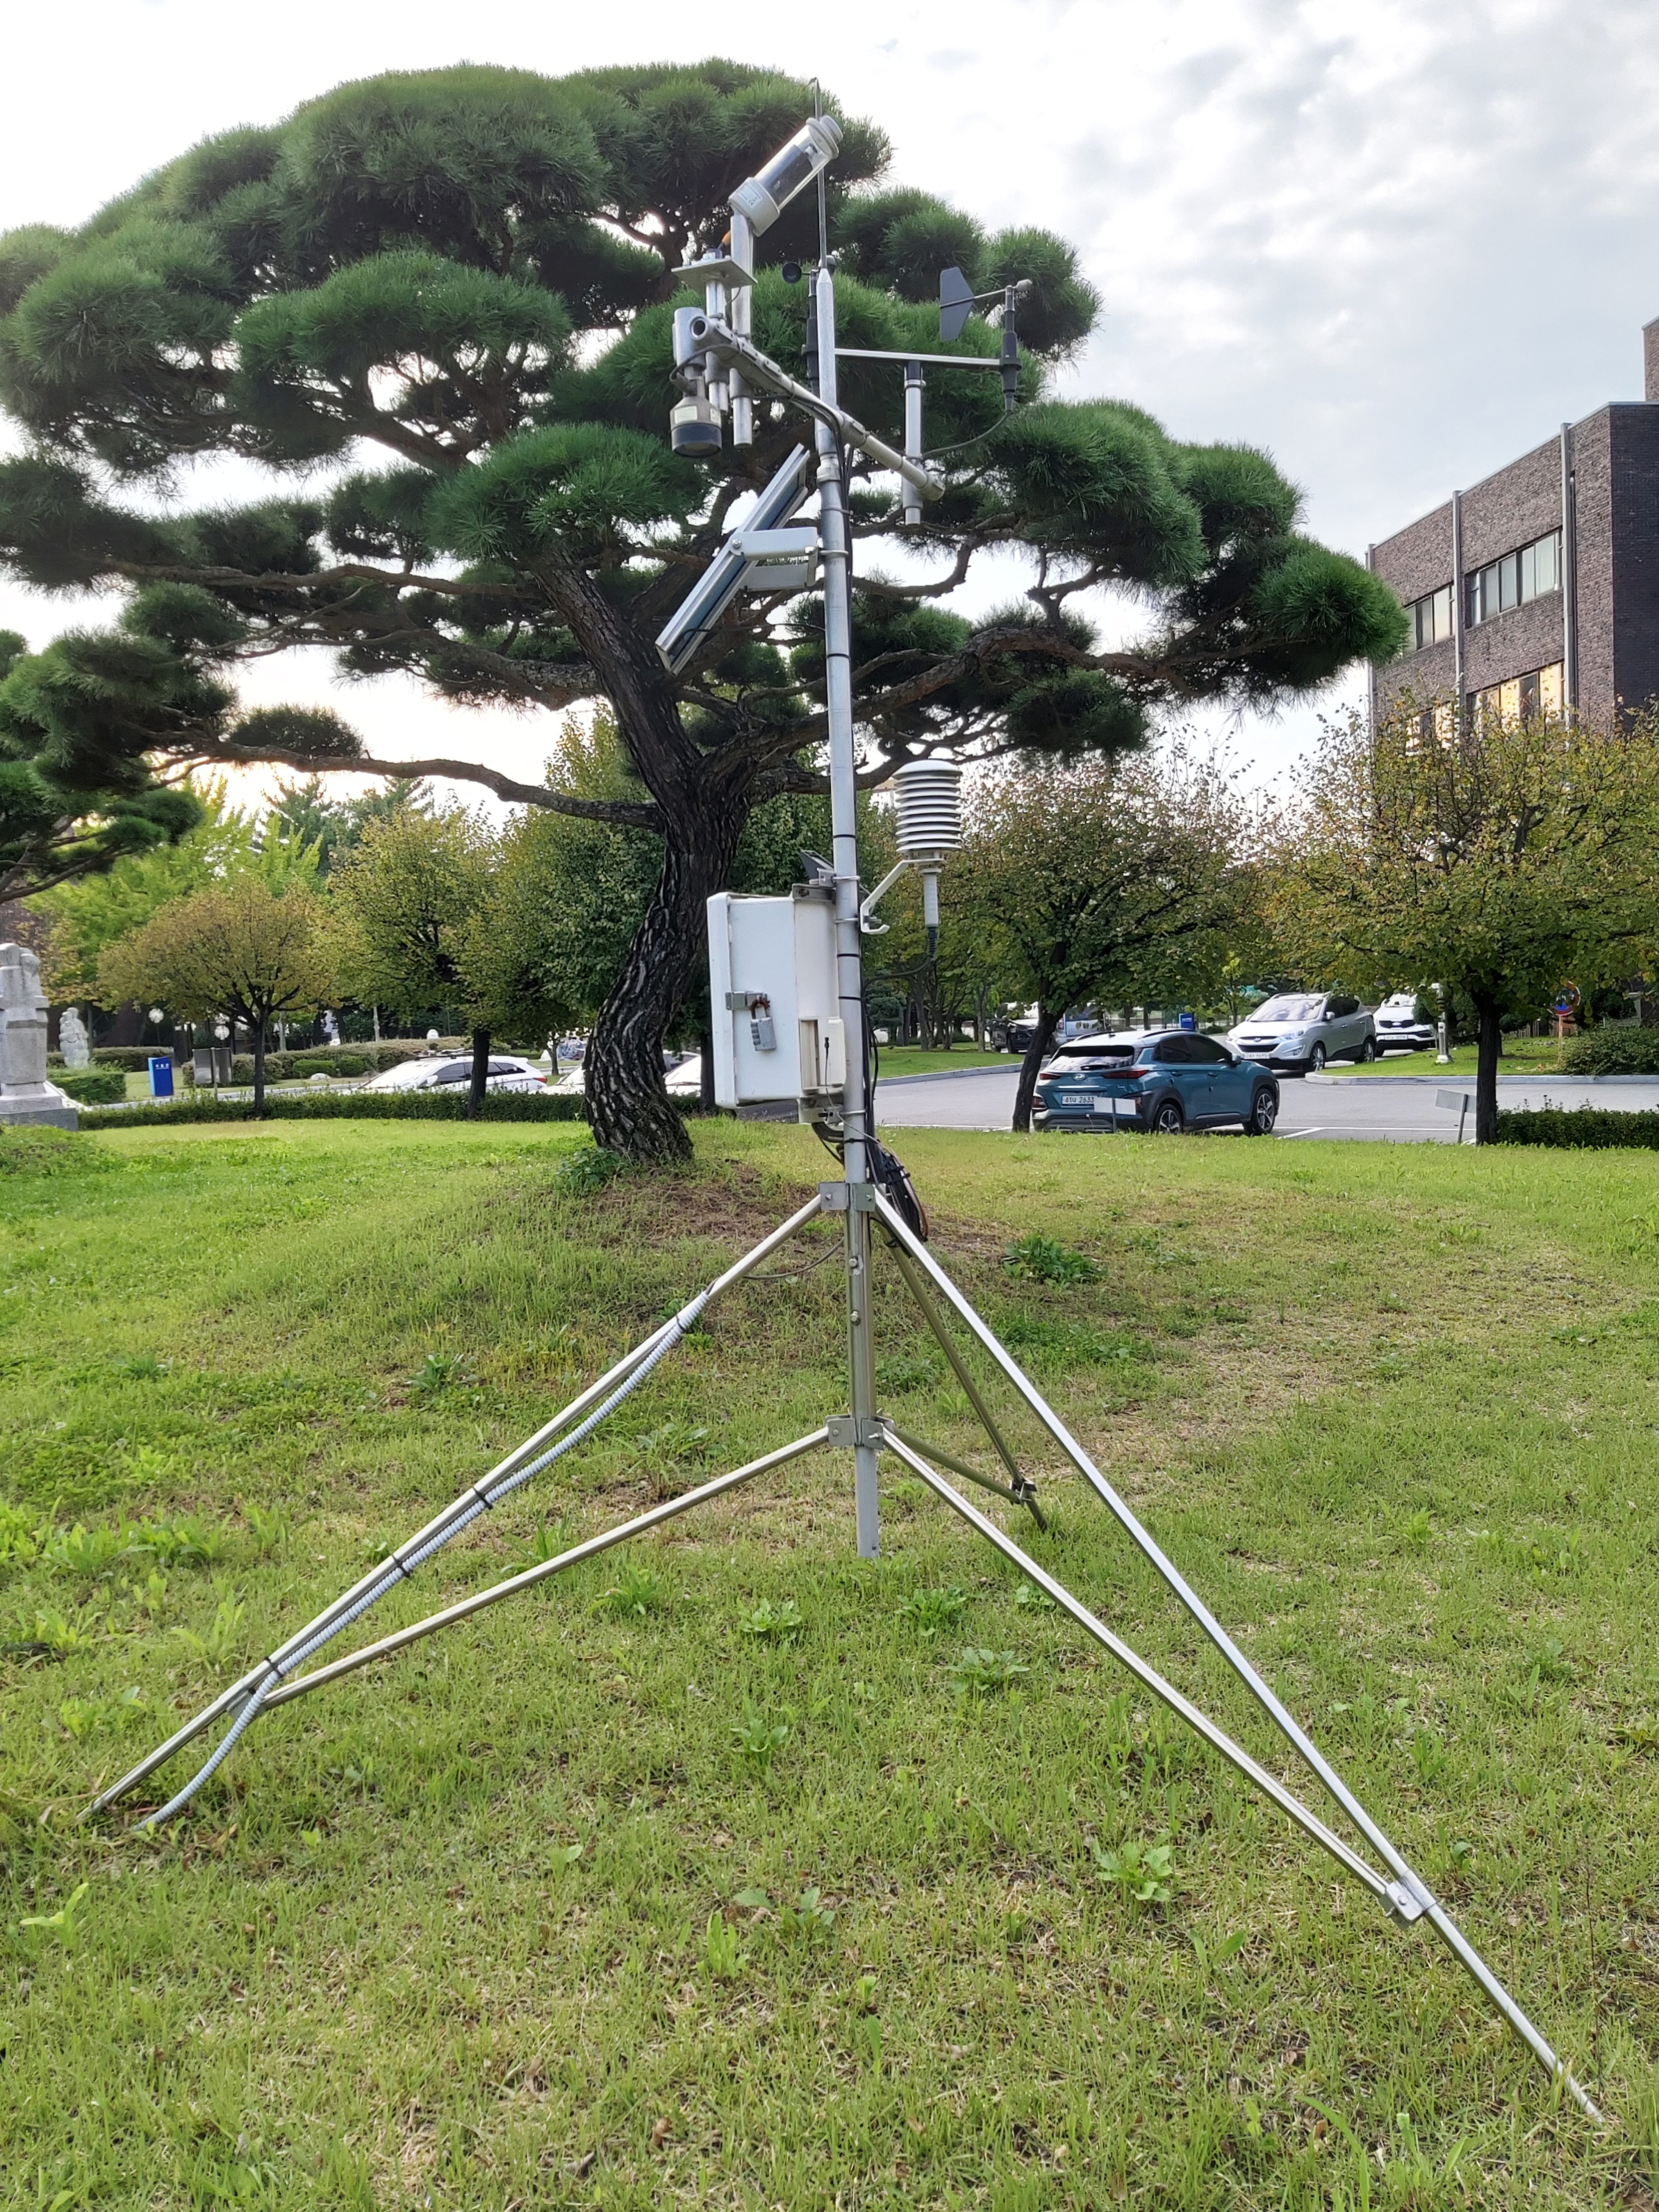
\includegraphics[width=.3\textwidth]{realaws}
	\caption{기상청 AWS 관측 자료와 한국교원대학교에 위치한 AWS 장치}
	\label{AWS}
\end{figure}